\documentclass[letter,11pt]{article}

\usepackage[spanish,es-nodecimaldot]{babel}
\usepackage[utf8]{inputenc}

\usepackage{lmodern}
\usepackage[T1]{fontenc}
\usepackage{textcomp}

\usepackage{framed}
\usepackage[svgnames]{xcolor}
\colorlet{shadecolor}{Gainsboro!50}

\usepackage[labelfont=bf]{caption}
\usepackage{graphicx}
\usepackage{pstricks}

\usepackage{anysize}
\marginsize{3cm}{2cm}{2cm}{3cm}

\usepackage{siunitx}
\usepackage{amsmath}
\usepackage{array}
\usepackage{csquotes}
\usepackage{steinmetz}

\usepackage{fancyhdr}
\usepackage{lastpage}
\pagestyle{fancy}
\fancyhf{}
\fancyhead[LE,RO]{Laboratorio de Circuitos Eléctricos III}
\fancyfoot[CO,CE]{\thepage\ de \pageref{LastPage}}

\special{papersize=215.9mm,279.4mm}

\usepackage[
    pdfauthor={Carlos Eduardo Caballero Burgoa},%
    pdftitle={Laboratorio de Circuitos Eléctricos III},%
    pdfsubject={Circuitos trifásicos desequilibrados con fuente estrella y carga estrella},%
    colorlinks,%
    citecolor=black,%
    filecolor=black,%
    linkcolor=black,%
    urlcolor=black,
    breaklinks]{hyperref}
\usepackage{breakurl}

\renewcommand{\arraystretch}{1.2}

\begin{document}

\begin{titlepage}
    \begin{center}
        {\Large UNIVERSIDAD MAYOR DE SAN SIMÓN}\\
        \vspace*{0.15cm}
        {\large FACULTAD DE CIENCIAS Y TECNOLOGÍA}\\
        \vspace*{0.10cm}
        DEPARTAMENTO DE ELÉCTRICA-ELECTRÓNICA\\
        \vspace*{3.0cm}
        {\Large \textbf{LABORATORIO DE CIRCUITOS ELÉCTRICOS III}}\\
        \vspace*{0.3cm}
        {\Large \textbf{INFORME No. 3}}\\
        \vspace*{3.5cm}
        {\Large \textbf{CIRCUITOS TRIFÁSICOS DESEQUILIBRADOS \\
        CON FUENTE ESTRELLA Y CARGA ESTRELLA}}\\
    \end{center}

    \vspace*{5.8cm}
    \leftskip=7.95cm
    \noindent
    \textbf{Estudiante:}\\
    Caballero Burgoa, Carlos Eduardo.\\
    \newline
    \textbf{Carrera:}\\
    Ing. Electromecánica.\\
    \newline
    \textbf{Docente:}\\
    Ing. Marco Antonio Vallejo Camacho.\\
    \newline
    \textbf{Grupo:} 2F (Martes).\\
\textbf{Fecha de entrega:} 2 de Octubre del 2024.\\
\end{titlepage}

\section{Cálculos teóricos}
Considerando un circuito trifásico estrella-estrella desequilibrado con las
siguientes cargas:

\begin{itemize}
    \item \textbf{Carga A}: $R_1=1[k\Omega]$.
    \item \textbf{Carga B}: $R_2=250[\Omega]$ y $L=1[H]$.
    \item \textbf{Carga C}: $R_3=500[\Omega]$ y $C=10[\mu F]$.
\end{itemize}

Con voltaje de fase $U_L=220[\text{V}]$ y con frecuencia de $50[\text{Hz}]$,
se hallan las corrientes de linea para los siguientes casos:
\\

\subsection{Sin linea de neutro}
\begin{figure}[!h]
\centering
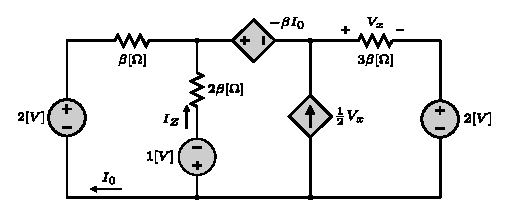
\includegraphics[scale=0.9]{figura1.eps}
\caption{Circuito trifásico desequilibrado sin linea de neutro.}
\label{simulacion1}
\end{figure}

\subsubsection{Secuencia positiva}
Se calcula la frecuencia angular ($\omega$):
\begin{equation*}
    \begin{split}
        \omega&=2\pi f\\
              &=2\pi(50)\\
              &=100\pi[\text{rad}/\text{s}]\\
    \end{split}
\end{equation*}

Se hallan las impedancias en el dominio de frecuencia:
\begin{equation*}
    \begin{split}
        Z_1 &= R_1\\
            &= 1000[\Omega]\\
    \end{split}
\end{equation*}

\begin{equation*}
    \begin{split}
        Z_2 &= R_2+j\omega L\\
            &= 250+j100\pi[\Omega]\\
    \end{split}
\end{equation*}

\begin{equation*}
    \begin{split}
        Z_3 &= R_3+\frac{1}{j\omega C}\\
            &= 500-j\frac{1000}{\pi}[\Omega]\\
    \end{split}
\end{equation*}

Considerando una secuencia positiva:
\begin{equation*}
    \begin{split}
        U_a = 220\phase{0^{\circ}}\,[\text{V}]\\
        U_b = 220\phase{-120^{\circ}}\,[\text{V}]\\
        U_c = 220\phase{120^{\circ}}\,[\text{V}]\\
    \end{split}
\end{equation*}

Se calcula el voltaje entre neutros con el teorema de \emph{Millman}:
\begin{equation*}
    \begin{split}
        U_0 &= \dfrac{
                   \dfrac{U_a}{Z_1}+\dfrac{U_b}{Z_2}+\dfrac{U_c}{Z_3}
               }{
                   \dfrac{1}{Z_1}+\dfrac{1}{Z_2}+\dfrac{1}{Z_3}
               }\\
            &= \dfrac{
                   \dfrac{220\phase{0^{\circ}}}{1000}+
                   \dfrac{220\phase{-120^{\circ}}}{250+j100\pi}+
                   \dfrac{120\phase{120^{\circ}}}{500-j(1000/\pi)}
               }{
                   \dfrac{1}{1000}+
                   \dfrac{1}{250+j100\pi}+
                   \dfrac{1}{500-j(1000/\pi)}
               }\\
            &= 159.99\phase{-173.20^{\circ}}[\text{V}]\\
    \end{split}
\end{equation*}

A partir del voltaje de neutro se calculan las corrientes de linea:
\begin{equation*}
    \begin{split}
        I_{L_1} &= \frac{U_a - U_0}{Z_1}\\
                &= \frac{200\phase{0^{\circ}}-159.99\phase{-173.20^{\circ}}}{500}\\
                &= 0.38\phase{2.86^{\circ}}[\text{A}]\\
    \end{split}
\end{equation*}
\begin{equation*}
    \begin{split}
        I_{L_2} &= \frac{U_b - U_0}{Z_2}\\
                &= \frac{200\phase{-120^{\circ}}-159.99\phase{-173.20^{\circ}}}{250+j100\pi}\\
                &= 0.44\phase{-125.59^{\circ}}[\text{A}]\\
    \end{split}
\end{equation*}
\begin{equation*}
    \begin{split}
        I_{L_3} &= \frac{U_c - U_0}{Z_3}\\
                &= \frac{200\phase{120^{\circ}}-159.99\phase{-173.20^{\circ}}}{500-j(1000/\pi)}\\
                &= 0.36\phase{109.35^{\circ}}[\text{A}]\\
    \end{split}
\end{equation*}
\\

\subsubsection{Secuencia negativa}
Considerando una secuencia negativa:
\begin{equation*}
    \begin{split}
        U_a = 220\phase{0^{\circ}}\,[\text{V}]\\
        U_b = 220\phase{120^{\circ}}\,[\text{V}]\\
        U_c = 220\phase{-120^{\circ}}\,[\text{V}]\\
    \end{split}
\end{equation*}

Se calcula el voltaje entre neutros con el teorema de \emph{Millman}:
\begin{equation*}
    \begin{split}
        U_0 &= \dfrac{
                   \dfrac{U_a}{Z_1}+\dfrac{U_b}{Z_2}+\dfrac{U_c}{Z_3}
               }{
                   \dfrac{1}{Z_1}+\dfrac{1}{Z_2}+\dfrac{1}{Z_3}
               }\\
            &= \dfrac{
                   \dfrac{220\phase{0^{\circ}}}{1000}+
                   \dfrac{220\phase{120^{\circ}}}{250+j100\pi}+
                   \dfrac{120\phase{-120^{\circ}}}{500-j(1000/\pi)}
               }{
                   \dfrac{1}{1000}+
                   \dfrac{1}{250+j100\pi}+
                   \dfrac{1}{500-j(1000/\pi)}
               }\\
            &= 111.57\phase{32.36^{\circ}}[\text{V}]\\
    \end{split}
\end{equation*}

A partir del voltaje de neutro se calculan las corrientes de linea:
\begin{equation*}
    \begin{split}
        I_{L_1} &= \frac{U_a - U_0}{Z_1}\\
                &= \frac{200\phase{0^{\circ}}-111.57\phase{32.36^{\circ}}}{500}\\
                &= 0.14\phase{-25.40^{\circ}}[\text{A}]\\
    \end{split}
\end{equation*}
\begin{equation*}
    \begin{split}
        I_{L_2} &= \frac{U_b - U_0}{Z_2}\\
                &= \frac{200\phase{-120^{\circ}}-111.57\phase{32.36^{\circ}}}{250+j100\pi}\\
                &= 0.60\phase{95.87^{\circ}}[\text{A}]\\
    \end{split}
\end{equation*}
\begin{equation*}
    \begin{split}
        I_{L_3} &= \frac{U_c - U_0}{Z_3}\\
                &= \frac{200\phase{120^{\circ}}-111.57\phase{32.36^{\circ}}}{500-j(1000/\pi)}\\
                &= 0.54\phase{-96.74^{\circ}}[\text{A}]\\
    \end{split}
\end{equation*}
\\

\subsection{Con linea de neutro}
\begin{figure}[!h]
\centering
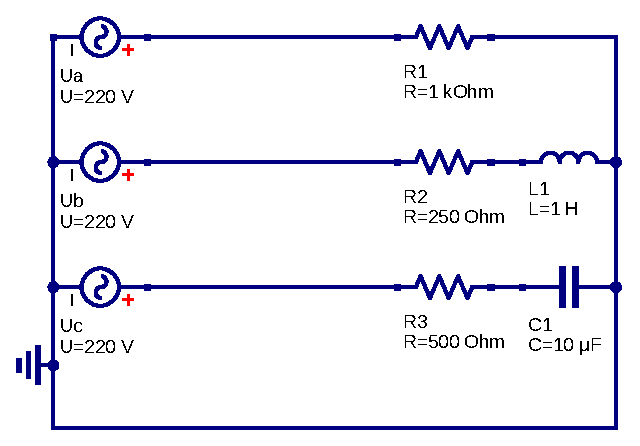
\includegraphics[scale=0.9]{figura2.eps}
\caption{Circuito trifásico desequilibrado con linea de neutro.}
\label{simulacion1}
\end{figure}

\subsubsection{Secuencia positiva}
Considerando una secuencia positiva:
\begin{equation*}
    \begin{split}
        U_a = 220\phase{0^{\circ}}\,[\text{V}]\\
        U_b = 220\phase{-120^{\circ}}\,[\text{V}]\\
        U_c = 220\phase{120^{\circ}}\,[\text{V}]\\
    \end{split}
\end{equation*}

Se calculan las corrientes de linea:
\begin{equation*}
    \begin{split}
        I_{L_1} &= \frac{U_a}{Z_1}\\
                &= \frac{200\phase{0^{\circ}}}{500}\\
                &= 0.22\phase{0^{\circ}}[\text{A}]\\
    \end{split}
\end{equation*}
\begin{equation*}
    \begin{split}
        I_{L_2} &= \frac{U_b}{Z_2}\\
                &= \frac{200\phase{-120^{\circ}}}{250+j100\pi}\\
                &= 0.55\phase{-171.49^{\circ}}[\text{A}]\\
    \end{split}
\end{equation*}
\begin{equation*}
    \begin{split}
        I_{L_3} &= \frac{U_c}{Z_3}\\
                &= \frac{200\phase{120^{\circ}}}{500-j(1000/\pi)}\\
                &= 0.37\phase{152.48^{\circ}}[\text{A}]\\
    \end{split}
\end{equation*}

Con las corrientes de linea se calcula la corriente de neutro:
\begin{equation*}
    \begin{split}
        I_0 &= U_{L_1}+U_{L_2}+U_{L_3}\\
            &= 0.22\phase{0^{\circ}}+0.55\phase{-171.49^{\circ}}+0.37\phase{152.48^{\circ}}\\
            &= 0.66\phase{172.10^{\circ}}[\text{A}]\\
    \end{split}
\end{equation*}
\\

\subsubsection{Secuencia negativa}
Considerando una secuencia negativa:
\begin{equation*}
    \begin{split}
        U_a = 220\phase{0^{\circ}}\,[\text{V}]\\
        U_b = 220\phase{120^{\circ}}\,[\text{V}]\\
        U_c = 220\phase{-120^{\circ}}\,[\text{V}]\\
    \end{split}
\end{equation*}

Se calculan las corrientes de linea:
\begin{equation*}
    \begin{split}
        I_{L_1} &= \frac{U_a}{Z_1}\\
                &= \frac{200\phase{0^{\circ}}}{500}\\
                &= 0.22\phase{0^{\circ}}[\text{A}]\\
    \end{split}
\end{equation*}
\begin{equation*}
    \begin{split}
        I_{L_2} &= \frac{U_b}{Z_2}\\
                &= \frac{200\phase{120^{\circ}}}{250+j100\pi}\\
                &= 0.55\phase{68.51^{\circ}}[\text{A}]\\
    \end{split}
\end{equation*}
\begin{equation*}
    \begin{split}
        I_{L_3} &= \frac{U_c}{Z_3}\\
                &= \frac{200\phase{-120^{\circ}}}{500-j(1000/\pi)}\\
                &= 0.37\phase{-87.52^{\circ}}[\text{A}]\\
    \end{split}
\end{equation*}

Con las corrientes de linea se calcula la corriente de neutro:
\begin{equation*}
    \begin{split}
        I_0 &= U_{L_1}+U_{L_2}+U_{L_3}\\
            &= 0.22\phase{0^{\circ}}+0.55\phase{68.51^{\circ}}+0.37\phase{-87.52^{\circ}}\\
            &= 0.46\phase{17.66^{\circ}}[\text{A}]\\
    \end{split}
\end{equation*}
\\

\subsection{Resumen de resultados}
\begin{center}
    \begin{tabular}{|c|c||c|c|c||c|c|}
    \hline
    \multicolumn{2}{|c||}{} &
    $I_{L_1}[\text{A}]$ & $I_{L_2}[\text{A}]$ & $I_{L_3}[\text{A}]$ & $U_0[\text{V}]$ & $I_0[\text{A}]$
    \tabularnewline \hline \hline
    $(+)$ & \textbf{SN} &
    $0.38\phase{2.86^{\circ}}$ &
    $0.44\phase{-125.59^{\circ}}$ &
    $0.36\phase{109.35^{\circ}}$ &
    $159.99\phase{-173.20^{\circ}}$ & $-$
    \tabularnewline \hline
    & \textbf{CN} &
    $0.22\phase{0^{\circ}}$ &
    $0.55\phase{-171.49^{\circ}}$ &
    $0.37\phase{152.48^{\circ}}$ &
    $0$ & $0.66\phase{172.10^{\circ}}$
    \tabularnewline \hline
    $(-)$ & \textbf{SN} &
    $0.14\phase{-25.40^{\circ}}$ &
    $0.60\phase{95.87^{\circ}}$ &
    $0.54\phase{-96.74^{\circ}}$ &
    $111.57\phase{32.36^{\circ}}$ & $-$
    \tabularnewline \hline
    & \textbf{CN} &
    $0.22\phase{0^{\circ}}$ &
    $0.55\phase{68.51^{\circ}}$ &
    $0.37\phase{-87.52^{\circ}}$ &
    $0$ & $0.46\phase{17.66^{\circ}}$
    \tabularnewline \hline
    \end{tabular}
\end{center}

\section{Simulación}
Se utilizó el software \emph{Electronic Workbench v5.12.} para simular
los circuitos, estos pueden verse en las figuras: (\ref{simulacion1}),
(\ref{simulacion2}), (\ref{simulacion3}), (\ref{simulacion4}),
(\ref{simulacion5}) y (\ref{simulacion6}).

%\begin{figure}[!h]
%\centering
%\includegraphics[scale=1.08]{simulacion/practica2.1.eps}
%\caption{Simulación del circuito resistivo.}
%\label{simulacion1}
%\end{figure}

%\begin{figure}[!h]
%\centering
%\includegraphics[scale=1.08]{simulacion/practica2.2.eps}
%\caption{Simulación del circuito resistivo-inductivo.}
%\label{simulacion2}
%\end{figure}

%\begin{figure}[!h]
%\centering
%\includegraphics[scale=1.08]{simulacion/practica2.3.eps}
%\caption{Simulación del circuito resistivo-capacitivo.}
%\label{simulacion3}
%\end{figure}

\section{Tablas y mediciones}
En las tablas siguientes, se presentan los resultados obtenidos con las
mediciones realizadas en laboratorio.

\subsection{Carga Resistiva}

\begin{center}
    \begin{tabular}{|c|c|c|}
    \hline
    $I_{L_1}$ & $I_{L_2}$ & $I_{L_3}$
    \tabularnewline \hline \hline
    $0.75[A]$ & $0.76[A]$ & $0.76[A]$
    \tabularnewline \hline
    \end{tabular}
\end{center}

\begin{center}
    \begin{tabular}{|c||c|c|c|}
    \hline
    & $Z_{1}$ & $Z_{2}$ & $Z_{3}$
    \tabularnewline \hline \hline
    $U_{\text{FASE}}$ & $225[V]$ & $227[V]$ & $225[V]$
    \tabularnewline \hline
    $I_{\text{FASE}}$ & $0.42[A]$ & $0.42[A]$ & $0.42[A]$
    \tabularnewline \hline
    \end{tabular}
\end{center}

\subsection{Carga Resistiva-Inductiva}

\begin{center}
    \begin{tabular}{|c|c|c|}
    \hline
    $I_{L_1}$ & $I_{L_2}$ & $I_{L_3}$
    \tabularnewline \hline \hline
    $0.70[A]$ & $0.71[A]$ & $0.71[A]$
    \tabularnewline \hline
    \end{tabular}
\end{center}

\subsection{Carga Resistiva-Capacitiva}

\begin{center}
    \begin{tabular}{|c|c|c|}
    \hline
    $I_{L_1}$ & $I_{L_2}$ & $I_{L_3}$
    \tabularnewline \hline \hline
    $0.73[A]$ & $0.74[A]$ & $0.74[A]$
    \tabularnewline \hline
    \end{tabular}
\end{center}

\begin{center}
    \begin{tabular}{|c||c|c|c|}
    \hline
    & $Z_{1}$ & $Z_{2}$ & $Z_{3}$
    \tabularnewline \hline \hline
    $U_{\text{FASE}}$ & $226[V]$ & $228[V]$ & $227[V]$
    \tabularnewline \hline
    $U_{\text{R}}$ & $219[V]$ & $217[V]$ & $216[V]$
    \tabularnewline \hline
    $U_{\text{C}}$ & $67.5[V]$ & $67[V]$ & $65.9[V]$
    \tabularnewline \hline
    $I_{\text{FASE}}$ & $0.42[A]$ & $0.42[A]$ & $0.41[A]$
    \tabularnewline \hline
    \end{tabular}
\end{center}

\section{Cuestionario}

\begin{enumerate}

\item \textbf{Los voltajes de fase medidos, ¿son perfectamente equilibrados? ¿A
qué se debe el desequilibrio?}

Los valores de los voltajes de fase medidos difieren levemente, considerando que
la variación máxima es de $2 [\text{V}]$ para una medición de $225 [\text{V}]$ o
superior, se puede considerar un error despreciable; causado por los
instrumentos de medición, al proceso de medida y al leve desbalance de las
cargas conectadas.

\item \textbf{Con los datos de laboratorio determine las relaciones entre
corrientes de linea y de fase. ¿Este factor cumple las relaciones establecidas
en teoría?. Explique las variaciones en ambos casos claramente si los hubiera.}

Considerando los siguientes datos obtenidos:
\begin{center}
    \begin{tabular}{|c||c|c||c|}
    \hline
    & \textbf{Corriente} & \textbf{Corriente} & \textbf{Relación}
    \tabularnewline
    & \textbf{de linea} & \textbf{de fase} & \textbf{$L/F$}
    \tabularnewline
    & \textbf{(Promedio)} & \textbf{(Promedio)} & 
    \tabularnewline \hline \hline
    \textbf{Carga resistiva} & $0.7567[A]$ & $0.42[A]$ & $1.8017$
    \tabularnewline \hline
    \textbf{Carga resistiva-inductiva} & $0.7067[A]$ & $0.4067[A]$ & $1.7376$
    \tabularnewline \hline
    \textbf{Carga resistiva-capacitiva} & $0.7367[A]$ & $0.4167[A]$ & $1.7679$
    \tabularnewline \hline
    \end{tabular}
\end{center}

La relación teórica de $\sqrt{3}\,(1.7321)$ varia ligeramente en las mediciones
de laboratorio con respecto a la teoría y a la simulación; nuevamente son
cantidades despreciables de error.

\item \textbf{Verificar con las tensiones medidas, la ley de voltajes de
\emph{Kirchhoff} en cada impedancia $R-L$ y $R-C$. Dibuje el diagrama fasorial
para cada caso y determine el ángulo de desface entre la tensión de fase en la
carga y la corriente de fase.}

\underline{$R-L$:}
\begin{equation*}
    \begin{split}
        \sum V &= 227\phase{0^{\circ}}+227\phase{-120^{\circ}}+225\phase{120^{\circ}}\\
               &= 2\phase{-60^{\circ}} \approx 0
    \end{split}
\end{equation*}

%\begin{figure}[!h]
%\centering
%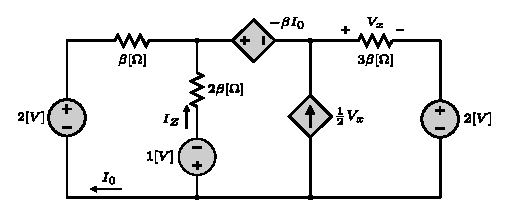
\includegraphics[scale=3.5]{figura1.eps}
%\caption{Diagrama fasorial para la suma de voltajes en $R-L$.}
%\end{figure}

\begin{equation*}
    \begin{split}
        I &=\frac{V}{Z}\\
          &=\frac{227\phase{0^{\circ}}}{500+j50\pi}\\
          &=0.433\phase{-17.44^{\circ}}[\text{A}]\\
    \end{split}
\end{equation*}

El \textbf{ángulo de desfase} es $-17.44^{\circ}$.

\underline{$R-C$:}
\begin{equation*}
    \begin{split}
        \sum V &= 226\phase{0^{\circ}}+228\phase{-120^{\circ}}+227\phase{120^{\circ}}\\
               &= 1.732\phase{-150} \approx 0
    \end{split}
\end{equation*}

%\begin{figure}[!h]
%\centering
%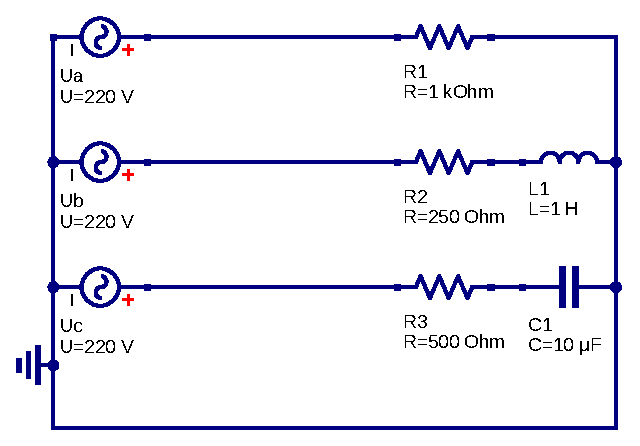
\includegraphics[scale=3.5]{figura2.eps}
%\caption{Diagrama fasorial para la suma de voltajes en $R-C$.}
%\end{figure}

\begin{equation*}
    \begin{split}
        I &=\frac{V}{Z}\\
          &=\frac{226\phase{0^{\circ}}}{500-j\frac{500}{\pi}}\\
          &=0.431\phase{17.66^{\circ}}[\text{A}]\\
    \end{split}
\end{equation*}

El \textbf{ángulo de desfase} es $17.66^{\circ}$.

\item \textbf{Investigue cuales son las ventajas y/o desventajas de este sistema
delta frente al sistema estrella.}

\underline{\textbf{Conexión estrella-estrella:}}

\underline{Ventajas}:
\begin{itemize}
    \item Posibilidad de sacar un neutro, lo cual permite obtener dos tensiones
        o bien conectar a tierra como medida de seguridad.
    \item Buen funcionamiento en pequeñas potencias.
\end{itemize}

\underline{Desventajas}:
\begin{itemize}
    \item Si las cargas en el circuito de transformador no están equilibradas,
        entonces los voltajes en las fases pueden llegar a desequilibrarse
        severamente.
\end{itemize}

\underline{\textbf{Conexión delta-delta:}}

\underline{Ventajas}:
\begin{itemize}
    \item No tiene desplazamiento de fase.
    \item No tiene problemas con cargas desequilibradas o armónicos.
\end{itemize}

\underline{Desventajas}:
\begin{itemize}
    \item No dispone de salida de neutro.
\end{itemize}

\end{enumerate}

\section{Conclusiones}
Se demostró experimentalmente la relación entre voltajes de linea y fase para 
un circuito trifásico fuente delta con carga delta equilibrada, comprobándose la
relación hallada en la teoría de circuitos eléctricos.

Se calcularon también las corrientes de linea y fase con diferentes impedancias
y también se comprobó que los valores teóricos, simulados, y hallados
experimentalmente no difieren mas allá de lo aceptable.

\begin{thebibliography}{99}

\bibitem{Rangel} Rangel, Stephani (2017, Octubre).\\
Ventajas y Desventajas de los diferentes tipos de conexiones para transformadores trifásicos.\\
Extraído el 24 de Septiembre del 2024, de:\\
https://es.scribd.com/document/362503390/Ventajas-y-Desventajas-de-Los-Diferentes-Tipos-de-Conexiones-Para-Transformadores-Trifasicos

\end{thebibliography}

\end{document}

